\input{pre}

\tikzset{rrail/.style={rground,yscale=-1}}
\newcommand{\reffig}[1]{Fig.~\ref{#1}}

\begin{document}
\input{frontpage}
\newpage
\section{Lab 7}
Fig.~1 shows a screenshot of the final layout with the padframe completed, and Fig.~2 the pre and post layout simulations of the
follower integrator.
\begin{figure}
    \center
    \includegraphics[width=\textwidth]{chip.png}
    \caption{Final layout of the delay line circuit with a padframe.}
    \label{}
\end{figure}
\begin{figure}
    \center
    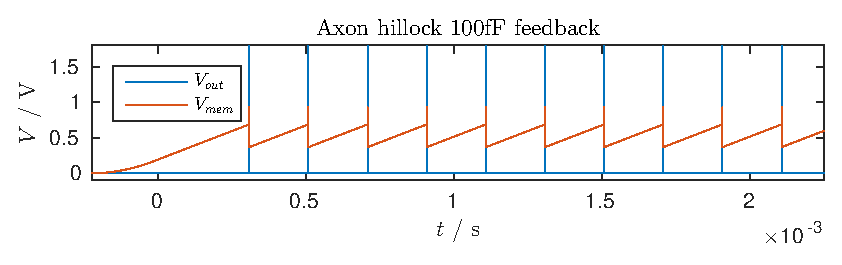
\includegraphics{fig1.eps}
    \caption{Pre and post layout AC simulation of a single follower integrator. Both of the circuits have a zero that 
    starts pulling the transfer function upwards for MHz frequencies, but the parasitic capacitance on the output transistor 
shifts the zero to a lower frequency for the post layout simulation.}
    \label{}
\end{figure}

\end{document}
